\chapter{Workshop Results}
\label{Chap:WorkshopResults}

The scope of the workshop is to evaluate the users mental models of the TonePrint Community, by describing how they imagine to use it for solving a specific task. As described in \autoref{WorkshopApproach} is concept maps used as a tool for the subjects, to depict their mental model for the context the task they have to solve. This results in Five different Concept maps describing Five different mental models for the individual task \autoref{TaskDecision}. \\
For the purpose of using the users mental models to shape the IA of the TonePrint Community, it's desired to look at similarities of the mental models. \textcite{WEB:ConceptMapAnalysis} suggest a method for analyzing a teams Shared Mental Model (SMM). SMM represents a mental model shared by a group of people working together i.e  at solving a problem or a task. It's important that there is a some what mutual consensus of the SMM, otherwise it would be difficult for the people working together, because they may not know the purpose of what their fellow team members do and it could cause miss communication. Even though the scope of this workshop isn't to evaluate a SMM regarding team members shared knowledge in order to work together, the scope of comparing mental models to find similarities is still valid. 

\section{Analysis Constructed Shared Mental Model}
\label{ACSMM}
To analyze the SMM it's proposed by \textcite{WEB:ConceptMapAnalysis} to create a Analysis Constructed Shared Mental Model (ACSMM). \autoref{fig:ACSMM} illustrates a very simplistic view of the process of constructing a ACSMM. At the beginning there is the users Individual Mental Model (IMM). These IMM is what is addressed in \autoref{MentalModel}. The next part is to acquire the users Individual Constructed Mental Model ICMM, which is their mental model putted in their own words. In this workshop the ICMM's is visualized be the concept maps created by each subject, as described in \autoref{WorkshopApproach}. The ICMM's is then analyzed and compared, so that a ASCMM may be created for explaining a common mental model shared by the users \autoref{fig:ACSMM}.  

\begin{figure}[H]
	\centering
	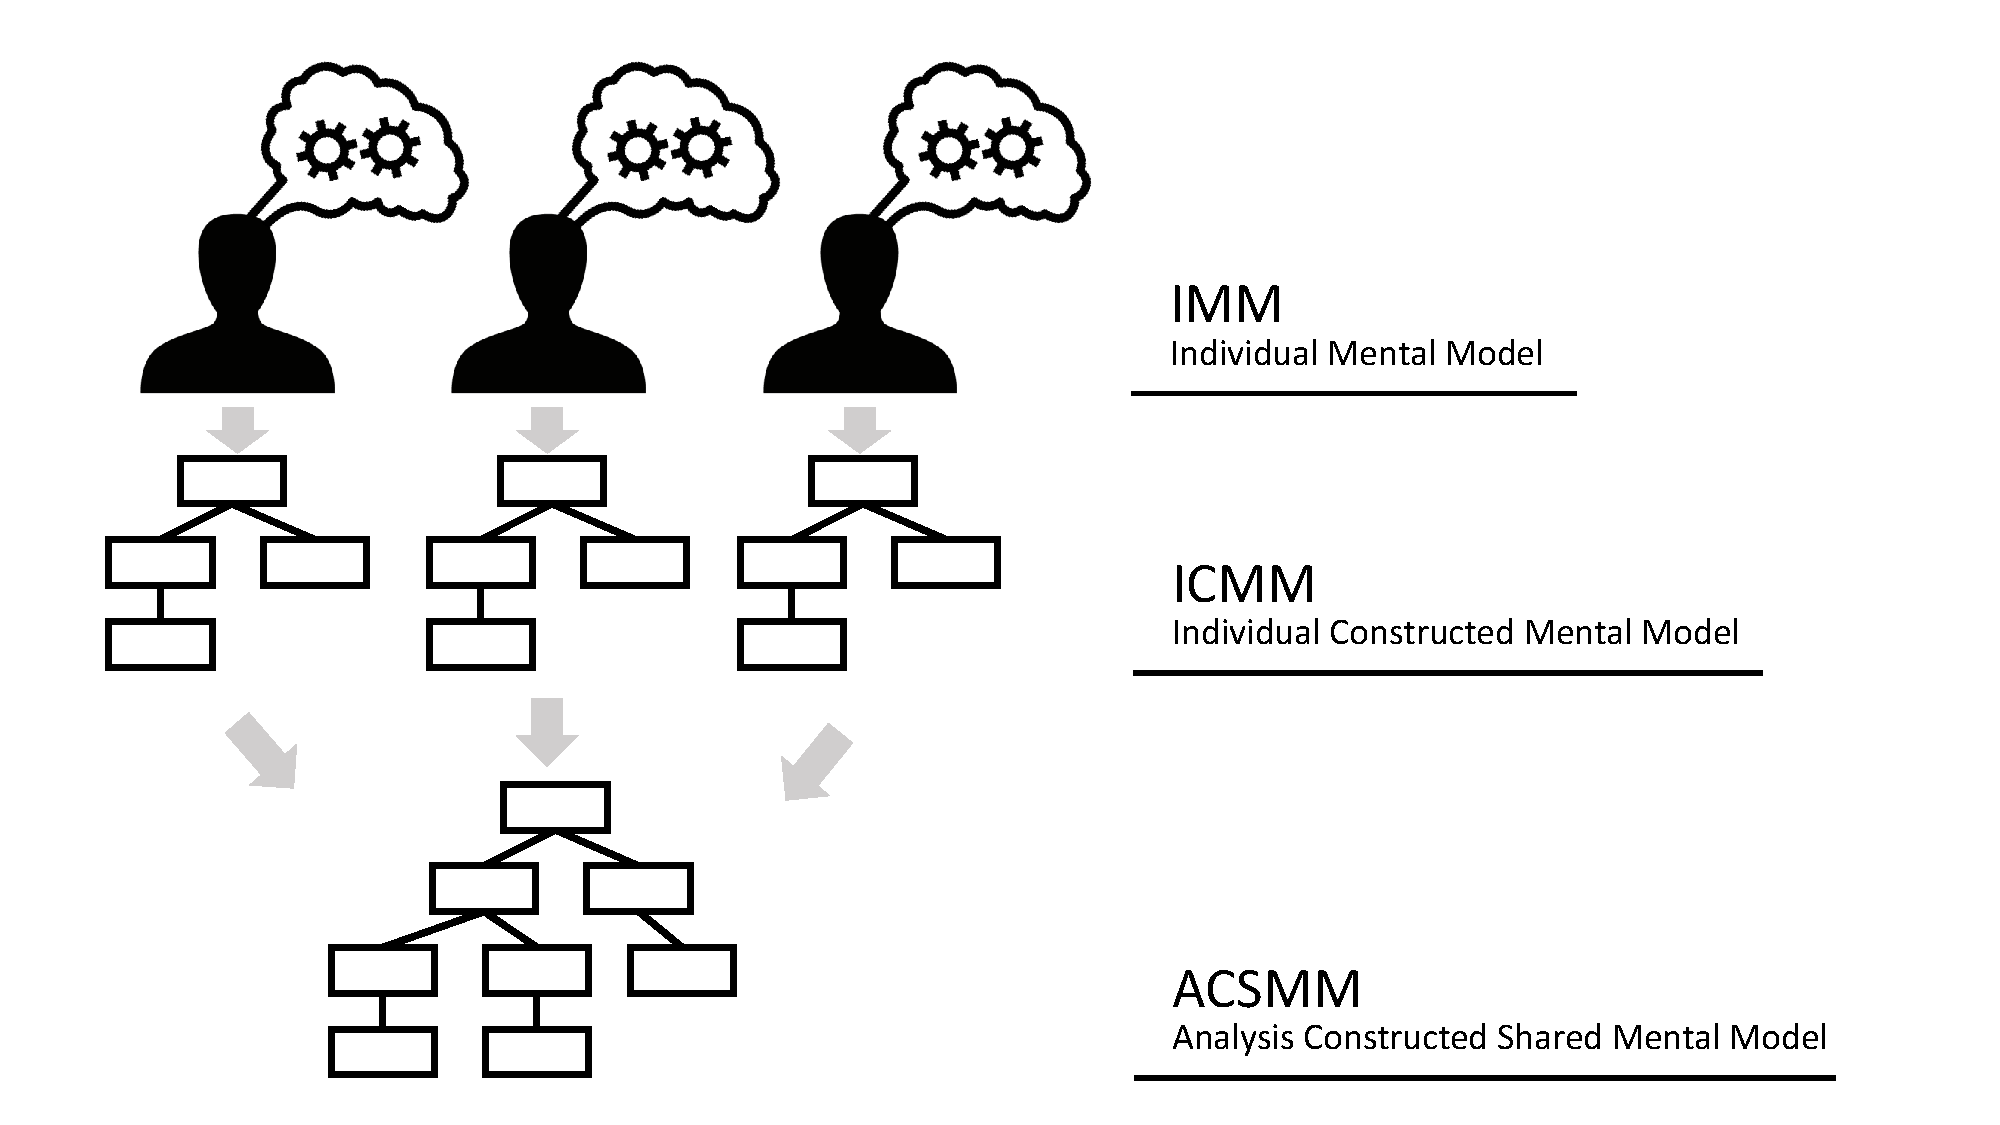
\includegraphics[width=\textwidth]{ACSMM.pdf}
	\caption{Illustration of the process of crating a ACSMM}
	\label{fig:ACSMM}
\end{figure}

The step of going from multiple ICMM to a ACSMM is described in \textcite{WEB:ConceptMapAnalysis} as a ICMM coding phase, a shared analysis phase and a SCSMM construction phase. In the coding phase the concepts, links and cluster depict in the ICMM's are transformed into code, that is easy comparable. The coding process for this workshop will not only be conducted for the subjects concept maps, however will it be based on the subjects presentation of their concept maps, which has been recorded \autoref{WorkshopApproach}. This is due to the concept maps being constructed quite different and because when putted to word, a more representative description of the IMM may be derived. In the shared analysis phase the codes from each subject is analyzed in order to determine which items of the ICMM's that the subjects shares. To determine this a criterion is set for percentages of subjects sharing an item. \textcite{WEB:ConceptMapAnalysis} suggest 50\% as criterion. Finally is the ACSMM constructed by taking the shared items from the previous step and use them to construct a Concept Map.

\subsection{Coding of the ICMM's}
\label{ICMMCoding}
The concept maps created by each subject is placed at the end of this chapter and is seen on \autoref{fig:ICMM1}, \autoref{fig:ICMM2}, \autoref{fig:ICMM3}, \autoref{fig:ICMM4} and \autoref{fig:ICMM5}. The content of the recorded descriptions given by each subject is represented independently in \autoref{Subject1ICMM} to \autoref{Subject5ICMM}. The concepts are highlighted with \textbf{Bold text} in the descriptions. The subjects codes are summarized in \autoref{tab:Subject1Coded} to \autoref{tab:Subject5Coded}.

\subsection{Shared Analysis}
\label{SharedAnalysis}
The lists containing the subjects individual codes, \autoref{tab:Subject1Coded} to \autoref{tab:Subject5Coded} are compared to each other to find the concepts which is shared. As recommended by \textcite{WEB:ConceptMapAnalysis} is the criterion for a concept to be identified as shared defined as 50\%. The concepts which is defined as shared is listed at \autoref{tab:SharedConcept}(WHich isn't finish). 

\begin{table}[H]
	\centering
	\begin{tabular}[width=\textwidth]{|l|c|}
	\hline
	Shared concept & Sharedness level (\%) \\ \hline
	TP App & 100\% \\ 
	User TonePrint Library & 60\% \\ \hline
	\end{tabular}
	\caption{Shared concepts and sharedness level}
	\label{tab:SharedConcept}
\end{table}


\subsubsection{Subject 1}
\label{Subject1ICMM}
\begin{figure}[H]
	\centering
	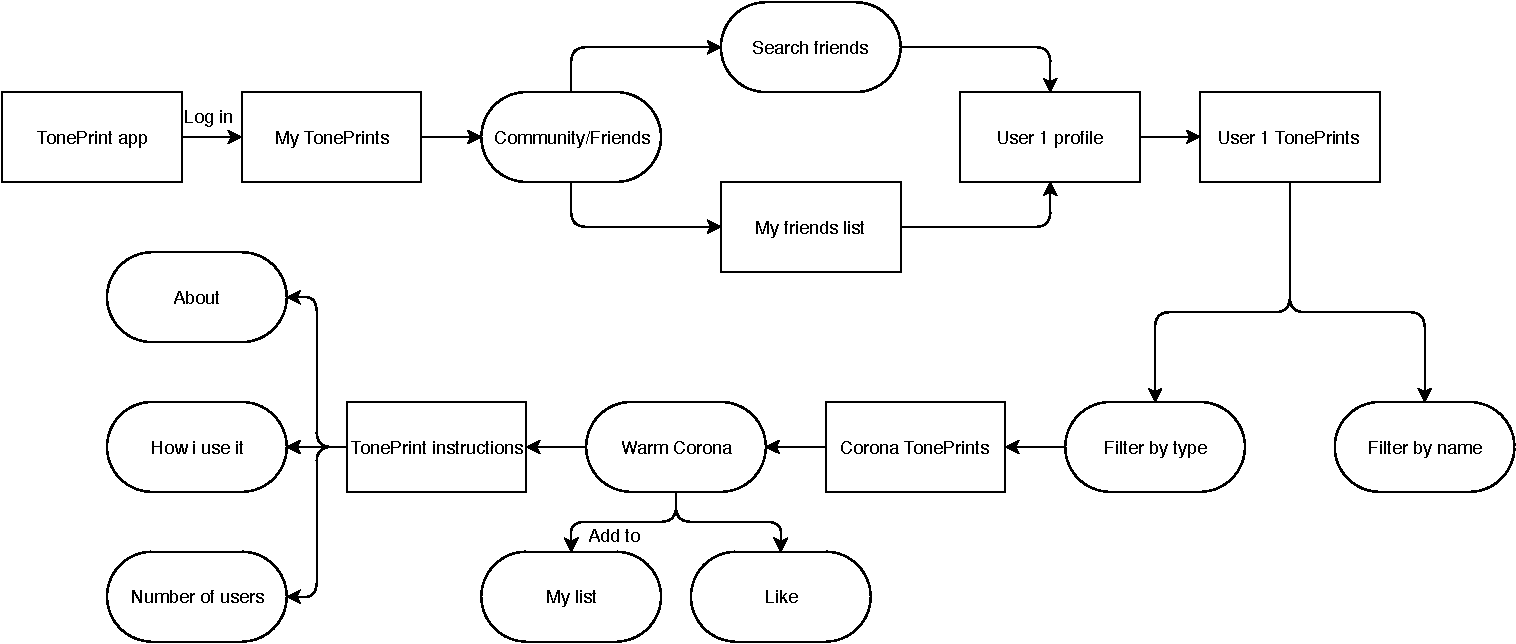
\includegraphics[width=0.6\textwidth]{1ICMM_new.pdf}
	\caption{The Concept map created by subject 1.}
	\label{fig:ICMM1}
\end{figure}

He begins at the \textbf{TP App} from which he wants to \textbf{Log in} If he isn’t already logged in. Than he enters his site \textbf{My TonePrints} which contains the buttons \textbf{Friends} and /or \textbf{Community}. He uses friends to either enter a \textbf{Search Friends} where he can find specific friends, or he enters \textbf{Friends List} where he gets an overview of all of his friends. He uses this to find/select user 1, hence entering \textbf{User 1 Profile}. On this profile he is presented a \textbf{List of TonePrints} created by user 1. The list is divided in \textbf{By Name} and \textbf{By Type}. From By Type he selects the Corona Type and is presented with a \textbf{Corona TP List}. From this list he’s able to use a checkbox saying \textbf{My List} which adds the TonePrint to his My TonePrints. There’s also a Gear/settings buttons, which he doesn’t know what does. He choses the \textbf{Warm Corona} TonePrint by clicking on the name, which presents him the \textbf{User 1 TP: Warm Corona} site. From this site he has the option to \textbf{Like} the TP, to se \textbf{Number of users using this} and read a description of \textbf{How I use It}.


\subsubsection{Subject 2}
\label{Subject2ICMM}
\begin{figure}[H]
	\centering
	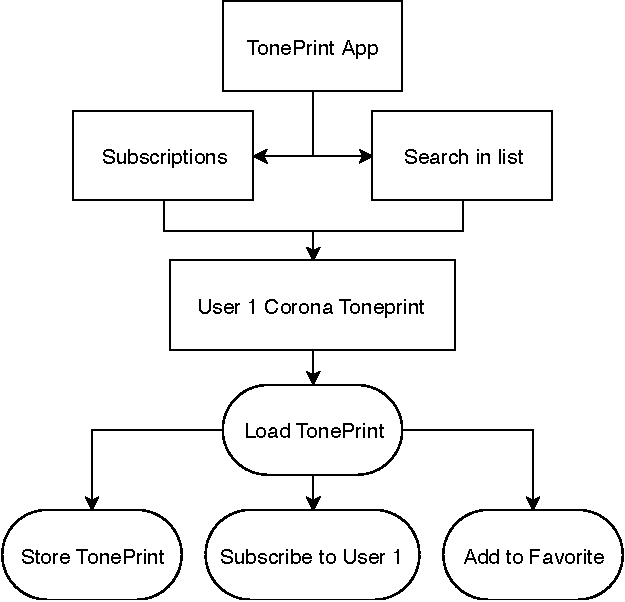
\includegraphics[width=0.4\textwidth]{2ICMM_new.pdf}
	\caption{The Concept map created by subject 2.}
	\label{fig:ICMM2}
\end{figure}

He begins by opening the \textbf{App}. He than have to opportunities, either he would open for his \textbf{Subscriptions} which is people he already subscribes, where he can find user 1, or he could go to another \textbf{list and search} for user 1. This list can be used for finding users who you don’t subscribe to. He then would Connect his pedal and guitar so that he can test the TP he’s about to find. He than go and chooses one of \textbf{User 1's Corona TonePrints} and \textbf{Loads it to his pedal}. He then tries the TP By playing he guitar. If he doesn’t like it, he would go find another. If he likes it he would like to have the option to \textbf{Subscribe to user 1} if he doesn’t already are a subscriber. He would also like the option to \textbf{Add the TonePrint as favorite}, so that it would be easier to find later. He than \textbf{Store the TonePrint} in his pedal. When he chooses to subscribe to user 1 he would like to have the option to select \textbf{Getting notification} either by mail or in app, when user 1 makes something new.

\subsubsection{Subject 3}
\label{Subject3ICMM}
\begin{figure}[H]
	\centering
	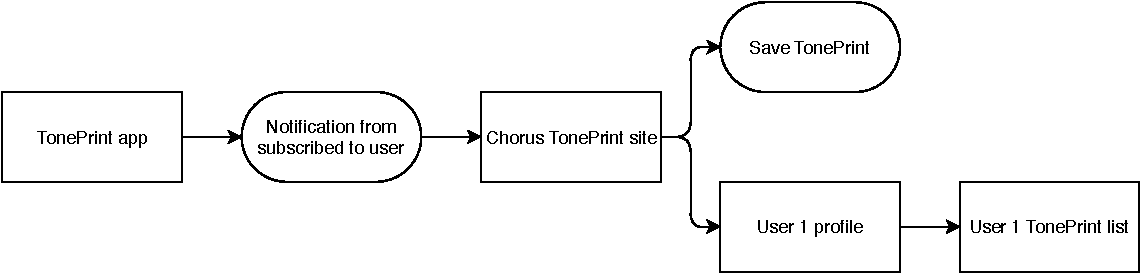
\includegraphics[width=0.4\textwidth]{3ICMM_new.pdf}
	\caption{The Concept map created by subject 3.}
	\label{fig:ICMM3}
\end{figure}

The first thing he does is to open the \textbf{TP App}. When it opens I gets a \textbf{Notification} telling that user 1, who he \textbf{subscribes} to have uploaded a new Chorus TonePrint. He than taps on the notification, which sends him to the \textbf{Specific Chorus TP Site}, in which he selects to \textbf{Save TonePrint}. He then gets the opportunity go to \textbf{User 1 Profile} where he can check the rest of \textbf{User 1’s TonePrints}, which he expect is given a \textbf{Logical indexation} which could be alphabetical or something else.

\subsubsection{Subject 4}
\label{Subject4ICMM}
\begin{figure}[H]
	\centering
	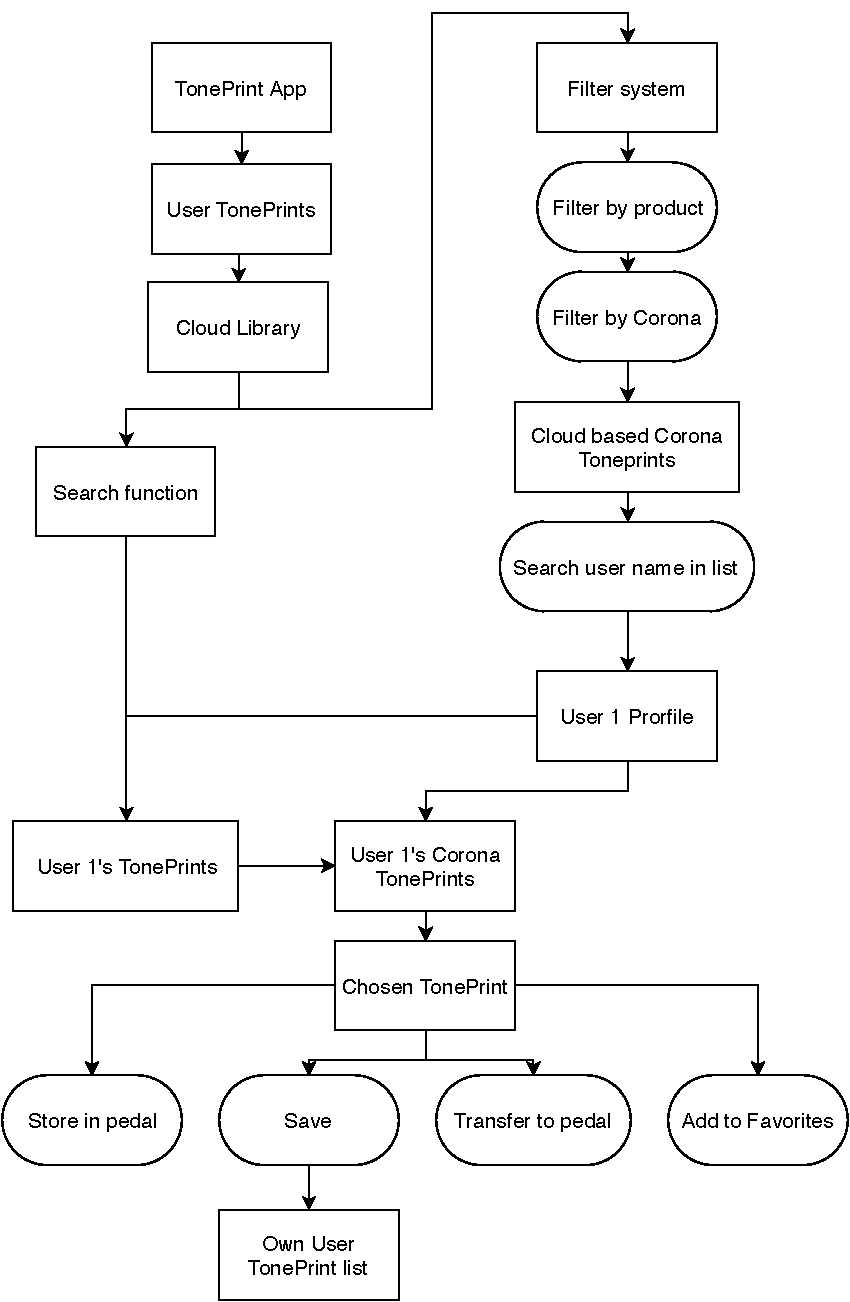
\includegraphics[width=0.4\textwidth]{4ICMM_new.pdf}
	\caption{The Concept map created by subject 4.}
	\label{fig:ICMM4}
\end{figure}

He begins by opening the \textbf{TP App} where expect it to have something like the currently infra structure. He navigates to the \textbf{User TonePrints} where he expects to find all of his own User TonePrints and the option to choose \textbf{Cloud Library} in which all the User Toneprints is stored. He chooses the Cloud Library because he wants to find a TonePrint from another user. Then goes to a \textbf{Filter system} where he wants to \textbf{Filter by product} where he chooses to \textbf{filter by Corona}. This presents him a list containing all \textbf{Cloud based Corona TonePrints}. Then he would be able to \textbf{Search for User names} in a \textbf{list} until he finds User 1. He also mentions another approach where instead of filtering use a \textbf{Search Function} to find all of \textbf{User 1’s TonePrints}. After his filtering and searching on User 1 he enters \textbf{User 1’s profile site} Containing all of his TonePrints, however just the ones for Corona, given the filtering. In this \textbf{User 1 Corona TonePrint list} he clicks on one so that he can try it, indicating he is \textbf{Transferring the TP to his pedal}. After trying it he then have the option to save it to his own \textbf{User Toneprint Library} and he’s in doubt what happens if he leaves the TonePrint, so he would also like to \textbf{Add it to Favorites}. He wants a interface like the current where he can \textbf{Save the TonePrint} and \textbf{Store it in pedal}.

\subsubsection{Subject 5}
\label{Subject5ICMM}
\begin{figure}[H]
	\centering
	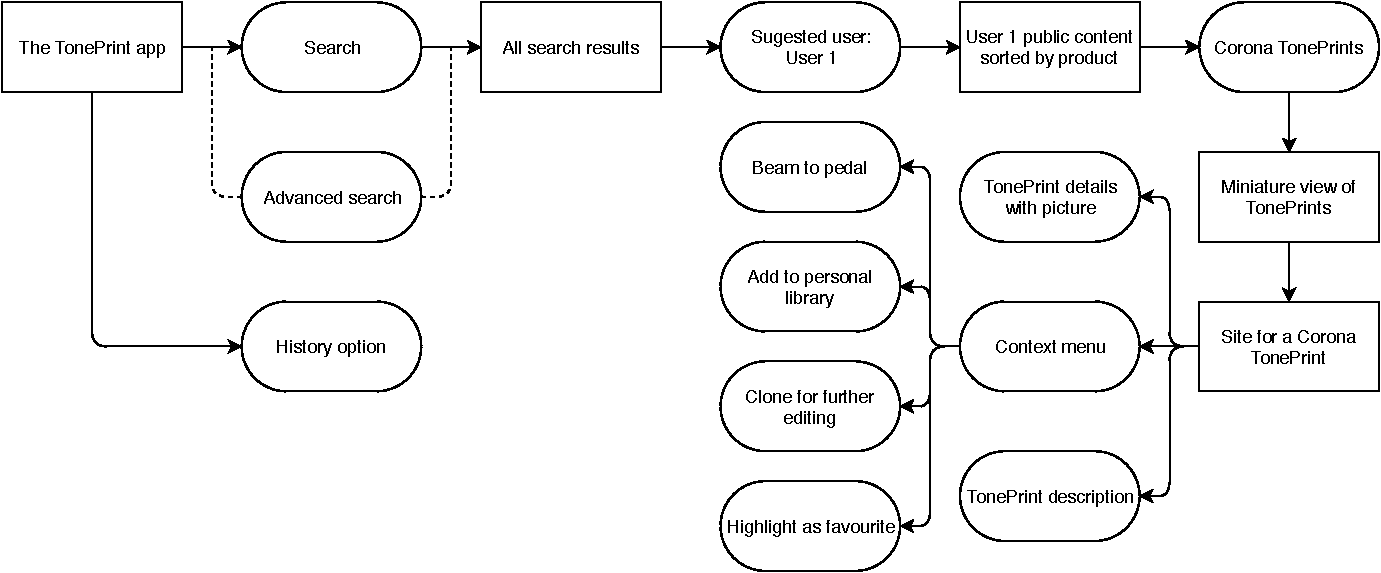
\includegraphics[width=0.4\textwidth]{5ICMM_new.pdf}
	\caption{The Concept map created by subject 5.}
	\label{fig:ICMM5}
\end{figure}

He wants the app to be simple and similar to some popular apps, so that it’s like something you have tried before. In the \textbf{TP App} he imagines a magnifying glass in the corner so that he can \textbf{Search}. He want to create a option for \textbf{Advanced Search}, where you can personalize what you are searching for, but also that the standard Search is a \textbf{Meta Search option}. This means that it search on ever thing int the system(TonePrints, User, Product…). He imagines that \textbf{Icons could indicate the category} of the search items. So when he searches User 1 it would \textbf{suggest User: User 1}. Then he comes to the \textbf{Public TonePrints by User 1}, which is \textbf{Lists organized by products}. From here he chooses a \textbf{Corona TP} from the \textbf{Corona list}. When selecting the TonePrint he’s presented with the \textbf{Toneprints details}, a \textbf{Picture} that has been attach and a \textbf{description}. If he just Right click or on the phone Hold he’s shown a \textbf{Context menu} where he can \textbf{Beam} the TonePrnt to his pedal, \textbf{Clone} it to his \textbf{Personal Library} where he can \textbf{edit it}, or \textbf{Favorite it} so it goes to his list of favorites. He want’s a \textbf{history function}, so even though he doesn’t save or favorites, he still have the option to backtrack to it, like in a web browser. 


\begin{table}[H]
\begin{minipage}[b]{0.5\linewidth}\centering

    \begin{tabular}{|l|}
    \hline
    Subject 1 \\ \hline
    TP App  \\
    Log in  \\
    My TonePrint site  \\
    Friends button  \\
    Community button  \\
    Search Friends  \\
    Friends List  \\
    User 1 Profile  \\
    User 1 TonePrint List  \\
    List by Name  \\
    List by Type  \\
    Corona TonePrint List  \\
    My List Check-box  \\
    Warm Corona TonePrint  \\
    User 1 TP: Warm corona site  \\
    Like  \\
    Number of users using this  \\
    How i use it  \\ \hline
    \end{tabular}
    \caption{List of subject 1's coded concepts}
    \label{tab:Subject1Coded}
    
	\begin{tabular}{|l|}
    \hline
    Subject 2 \\ \hline
    App \\
    Subscriptions  \\
    Search in List  \\
    User 1's Corona TonePrints  \\
    Load to Pedal  \\
    Subscribe to user 1  \\
    Add TonePrint to favorites  \\
    Store in Pedal  \\
    Getting notification  \\ \hline
    \end{tabular}
	\caption{List of subject 2's coded concepts}
    \label{tab:Subject2Coded}    
    
    \begin{tabular}{|l|}
    \hline
    Subject 3 \\ \hline
    TP App \\
    Notification  \\
    Subscribes  \\
    Specific Chorus TP site \\
    Save TonePrint \\
    User 1 Profile \\
    User 1's TonePrints \\
    Logical Indexation  \\ \hline
    \end{tabular}
	\caption{List of subject 3's coded concepts}
    \label{tab:Subject3Coded}
    
\end{minipage}
\begin{minipage}[b]{0.49\linewidth}\centering

    \begin{tabular}{|l|}
    \hline
    Subject 4 \\ \hline
    TP App \\
    User TonePrints \\
    Cloud Library \\
    Filter system \\
    Filter by product \\
    Filter by Corona \\
    Cloud based Corona TonePrints \\
    Search User Name \\
    Users List \\
    Search function \\
    User 1's TonePrints \\
    User 1 profile site \\
    User 1 Corona TonePrint \\
    Transfer to pedal \\
    Own User TonePrint Library \\
    Add to Favorites \\
    Save TonePrint \\
    Store in pedal  \\ \hline
    \end{tabular}
	\caption{List of subject 4's coded concepts}
    \label{tab:Subject4Coded}    
    
	\begin{tabular}{|l|}
    \hline
    Subject 5 \\ \hline
    TP App \\
   	Search  \\
    Advanced Search  \\
    Meta Search option  \\
    Icons indicating category  \\
    Suggest User: user 1  \\
    Public TonePrints by User 1  \\
    List organized by Products  \\
    Corona TonePrint \\
    Corona List \\
    TonePrints Details \\
    Picture \\
    Description \\
    Context Menu \\
    Beam \\
    Clone \\
    Personal Library \\
    Edit \\
    Favorite it \\
    History function  \\ \hline
    \end{tabular}
	\caption{List of subject 5's coded concepts}
    \label{tab:Subject5Coded}
        
\end{minipage}
\end{table}













